\section{Hilti Auspressgerät}
\label{Kapitel:Auspressgeraet}
Die von Hilti hergestellten chemischen Due;bel werden mit einem eigens dafue;r entwickelten Auspressgerae;t in gebohrte Loe;cher gedrue;ckt. Dieses Auspressgerae;t soll gleichzeitig moe;glichst zuverlae;ssig und stabil sein, aber auch so konstruiert dass fue;r die Anwendung wenig Kraft gebraucht wird und exakt so viel Fluid ausgepresst wird wie vom Anwender gewollt.\\
Das derzeit auf dem Markt erhae;ltliche Gerae;t ist in Abbildung \ref{fig:Auspressgeraet} gezeigt.
%
\begin{figure}
    \centering
    \subfigure[Handgerae;t]{
        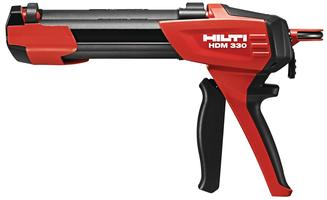
\includegraphics[width=0.31\textwidth]{figures/Auspressgeraet.jpg}
        \label{fig:Auspressgeraet:subA}
    }
    \subfigure[Akkugerae;t]{
        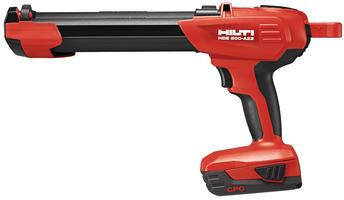
\includegraphics[width=0.31\textwidth]{figures/AuspressgeraetAkku.jpg}
        \label{fig:Auspressgeraet:subB}
    } 
    \subfigure[Moe;rtel Kartusche]{
        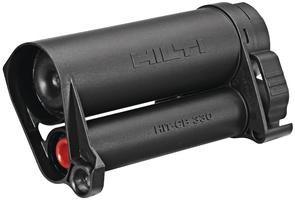
\includegraphics[width=0.31\textwidth]{figures/AuspressgeraetKasette.jpg}
        \label{fig:Auspressgeraet:subC}
    }
    \caption{Das Gerae;t zum Auspressen von Hilti Injektionsmoe;rtel. In \subref{fig:Auspressgeraet:subA} ist das Handgerae;t zu sehen, in \subref{fig:Auspressgeraet:subB} die Ausfue;hrung mit Akku, bei der das Auspressen auf Knopfdruck geschieht.\\
    In \subref{fig:Auspressgeraet:subC} ist eine Kartusche abgebildet, in die die Moe;rtelbeutel gelegt werden.}
    \label{fig:Auspressgeraet}
\end{figure}
%

Da die verwendeten Moe;rtel jeweils aus zwei Komponenten bestehen, mue;ssen sie bei der Anwendung gemischt werden. Dies geschieht in einem Mischer, der vorne am Auspressgerae;t angeschraubt wird. (Abbildung \ref{fig:Mischer})\\
%
\begin{figure}
    \centering
    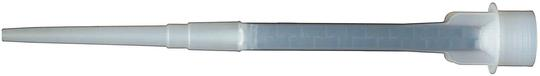
\includegraphics[width=0.8\textwidth]{figures/Mischer.jpg}
    \caption{Das Mischermodell HIT-RE-M, in dem die Moe;rtel nach dem Auspressen gemischt werden.}
    \label{fig:Mischer}
\end{figure}
%
Dieser Mischer kann jeweils nur einmal verwendet werden, weil der Moe;rtel ab dem Zeitpunkt des Mischens beginnt sich zu erhae;rten und so beginnt den Mischer zu verstopfen sobald das Auspressen gestoppt wird. Es ist deshalb im Interesse des Verbrauchers, dass der Mischer im Erwerb sehr preiswert ist. Trotzdem soll er natue;rlich die Komponenten moe;glichst gut mischen, da dies entscheidend fue;r die maximale Zuglast der Due;bel ist.

Diese Ansprue;che an das Gerae;t und den Mischer erfordern ein hohes Mass an Verstae;ndnis fue;r die Vorgae;nge wae;hrend dem Auspressen, weshalb sie in der Forschungsabteilung von Hilti stae;ndig weiter vermessen, simuliert und verbessert werden.
%
\subsection{Messaufbau}
Das fue;r die Moe;rtel verwendete Auspressgerae;t besteht zum groe;ssten Teil aus Kunststoff. Da dieser selber elastische Eigenschaften besitzt, ist es sehr schwierig die viskoelastischen Eigenschaften eines Fluides zu bestimmen, das durch das Geraet fliesst.\\
Um einen Einfluss des Gerae;tes auf das Fluid auszuschliessen, wurde deshalb die Geometrie des Auspressgerae;tes in einer sogenannten Funktionsersatzprue;fung (FEP) aus Metall nachgebaut. In Abbildung \ref{fig:FEP} sind Bilder dieser FEP zu sehen.
%
\begin{figure}
    \centering
    \subfigure[Metallnachbau]{
        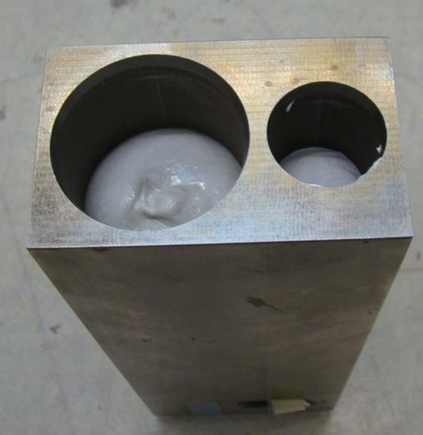
\includegraphics[width=0.31\textwidth]{figures/FEP_1.png}
        \label{fig:FEP:subA}
    }
    \subfigure[mit Moe;rtel gefue;llt]{
        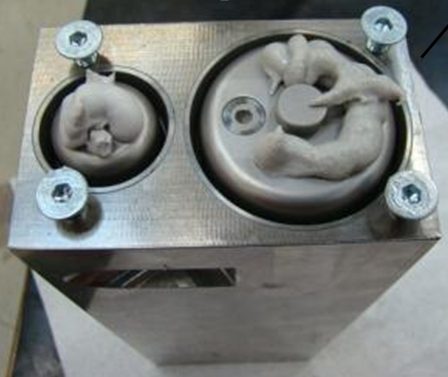
\includegraphics[width=0.31\textwidth]{figures/FEP_2.png}
        \label{fig:FEP:subB}
    } 
    \subfigure[Übergang zwischen Kolben und Mischer]{
        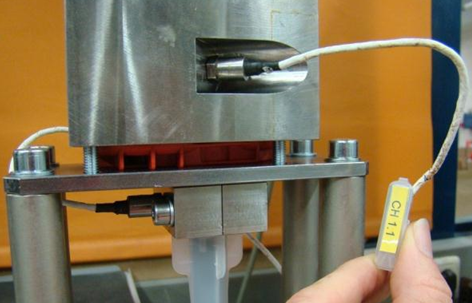
\includegraphics[width=0.31\textwidth]{figures/FEP_3.png}
        \label{fig:FEP:subC}
    }
    \caption{Der Messaufbau fue;r das Auspressgerae;t. In Abbildung \subref{fig:FEP:subA} ist der Nachbau der Geometrie aus Metall zu sehen, der in \subref{fig:FEP:subB} mit Moe;rtel befue;llt worden ist.\\
    Dieser Moe;rtel wird dann von einem Kolben durch eine Blende in den Mischer gepresst, der Übergang ist in \subref{fig:FEP:subC} zu sehen.}
    \label{fig:FEP}
\end{figure}
%
\subsection{Simulation}
\begin{todocontent}
    \1 Verwendete Netze
    \1 Loeserparameter (Relaxation)
    \1 Anfangsloesung wichtig fuer Konvergenz
\end{todocontent}
%
\subsection{Resultate}
\begin{todocontent}
    \1 Resultat Simulation (Bilder)
    \1 Druckvergleich
    \1 Einfluss Viskoelastizitaet
\end{todocontent}
